\icode{N14J-MI-SI-L2-261102-001}
\nceeID[unkown]{2014天津}{unknown}
如图所示，小球用细绳系住，绳的另一端固定于\(O\)点。现用水平力\(F\)缓慢推动斜面体，小球在斜面上无摩擦地滑动，细绳始终处于直线状态，当小球升到接近斜面顶端时细绳接近水平，此过程中斜面对小球的支持力\(F_N\)以及绳对小球的拉力\(F_T\)的变化情况是\paren[]

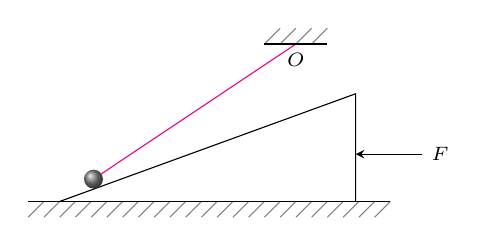
\begin{tikzpicture}[>=stealth,font=\scriptsize]
	\begin{scope}[rotate=20]
		\coordinate (O) at(.5,.12);
		\draw (0,0)--(4,0)--++(-110:{4*sin(20)});
	\end{scope}
	\draw[magenta] (O)--(3,2);
	\node at(3,1.8){\(O\)};
	\shade[ball color=gray] (O) circle(.12);
	\draw[->] (4.6,.6)node[right]{\(F\)}--(20:4|-4.6,.6);
	\foreach \x in {-.4,-.2,...,4}
		\draw[gray] (\x,-.2)--++(.2,.2);
	\foreach \x in {2.6,2.8,...,3.2}
		\draw[gray] (\x,2)--++(.2,.2);
	\draw (-.4,0)--(4.2,0) (2.6,2)--(3.4,2);
\end{tikzpicture}
\begin{choices}
	\item\(F_N\)保持不变，\(F_T\)不断增大
	\item\(F_N\)不断增大，\(F_T\)不断减小
	\item\(F_N\)保持不变，\(F_T\)先增大后减小
	\item\(F_N\)不断增大，\(F_T\)先减小后增大
\end{choices}
\begin{answer}
    B\qquad 提示：绳的极限情况是与斜面平行，所以\(F_T\)与\(F_N\)最终垂直

\begin{tikzpicture}[>=stealth,font=\scriptsize]
	\begin{scope}[rotate=20]
		\coordinate (O) at(.5,.12);
		\draw[gray] (0,0)--(4,0)--++(-110:{4*sin(20)});
	\end{scope}
	\draw[gray] (O)--(3,2);
	\node at(3,1.8){\(O\)};
	\shade[ball color=gray!50] (O) circle(.12);
    \draw[->] (O)--++(0,-1.5);
    \draw[->,magenta] (O)--++($.3*($(3,2)-(O)$)$)node[above]{\(F_T\)};
    \draw[->,teal] (O)--++(110:1.2)node[left]{\(F_N\)};
    \draw[->,dashed,magenta] ($(O)+(0,-1.5)$)--++($.185*($(3,2)-(O)$)$)coordinate(t);
    \draw[->,dashed,teal] (t)--(O);
	\draw[->,gray] (4.6,.6)node[right]{\(F\)}--(20:4|-4.6,.6);
	\foreach \x in {-.4,-.2,...,4}
		\draw[gray!50] (\x,-.2)--++(.2,.2);
	\foreach \x in {2.6,2.8,...,3.2}
		\draw[gray!50] (\x,2)--++(.2,.2);
	\draw[gray] (-.4,0)--(4.2,0) (2.6,2)--(3.4,2);
\end{tikzpicture}
\end{answer}